% -----------------------------------------------------------------------------
% November, 2023 update by Eve Torrence
% This file contains a sample Bridges paper in LaTeX format.
% The original was written by Carlo S\'equin in 2017, using previous
% versions by Doug McKenna, Craig Kaplan, Reza Sarhangi, and others,
% with \LaTeX\ contributions by Bruce Torrence and David Swart.
% It has been vetted using TeXShop 5.10 on Mac OS Big Sur (11.6).
% TeXShop is part of the TeX Live distribution, available
% at http://www.tug.org/texlive/
%
% -----------------------------------------------------------------------------

\documentclass[letterpaper,11pt]{article}
\usepackage{amsmath, amsthm, amssymb}    % May not all be necessary
\usepackage{bridges}			% Custom bridges proceedings style
\usepackage{graphicx}			% For including pictures
\usepackage[colorlinks=true, urlcolor=blue, citecolor=black, linkcolor=black]{hyperref}  
							% For formatting (clickable) URLs
\usepackage{subcaption}			% For captioning multi-panel figures

\urlstyle{rm} 					% Display URLs in same font as body text

% -----------------------------------------------------------------------------

\title{Simulating Digital Circuits Using Wang Cubes [under construction]}

\author{Mathew Kuthur James\textsuperscript{1}
\vspace{10pt}\\
\textsuperscript{1}David Cheriton School of CS, University of Waterloo} % end \author
% superscripts are only needed if there is more than one author

% \date{[Draft as of \today]}	% uncomment to use for your own draft purposes
\date{}					% Suppress any date on submissions

% -----------------------------------------------------------------------------

\begin{document}

\maketitle

% Prevent page number 1 from being printed on the first page.
\thispagestyle{empty}

\begin{abstract}

This report describes a method by which Wang cubes tiling 3D space can be used to simulate digital circuits, and presents a web-app to run such simulations. It also describes an efficient algorithm used to compute adjacent planes along the z-axis, along with the software architecture and technology used to create the web-app. Common elements of digital circuits (such as clocks, wires, logic gates, \emph{et cetera}), along with the challenges of instantiating them using Wang cubes, are discussed here.

\end{abstract}

% Bridges papers are usually no more than 8 pages in length.  So
% there's really no need to have numbered sections, unless the
% author really needs to refer to sections by number within the paper's text.  
% So to suppress sequential section numbers, append an asterisk to 
% the \section command, as in:

\section*{Introduction}

The primary goal of this project is to develop software to design and tile $R^3$ with Wang cubes, which are the 3D analogue for Wang tiles. Since 2D Wang tiles are Turing-complete, 3D Wang tiles possesses the expressive power required to simulate a Von Neumann machine built out of simple circuit elements like clocks, wires, logic-gates and flip-flops. 

Movement along the z-axis is treated as equivalent to stepping forward and backward in time, which is treated as a distinct quantity. At each stage, the current plane contains a finite number of tiles, which are used to compute the preceding and succeeding plane in real time. The algorithm to do so is described in this report. A user manual \cite{manual}, the web-app \cite{web-app}, its source \cite{web-app-source} and files describing common circuit elements \cite{wang-file} are available online.


\section*{Architecture}

\begin{figure}[h!tbp]
	\centering
	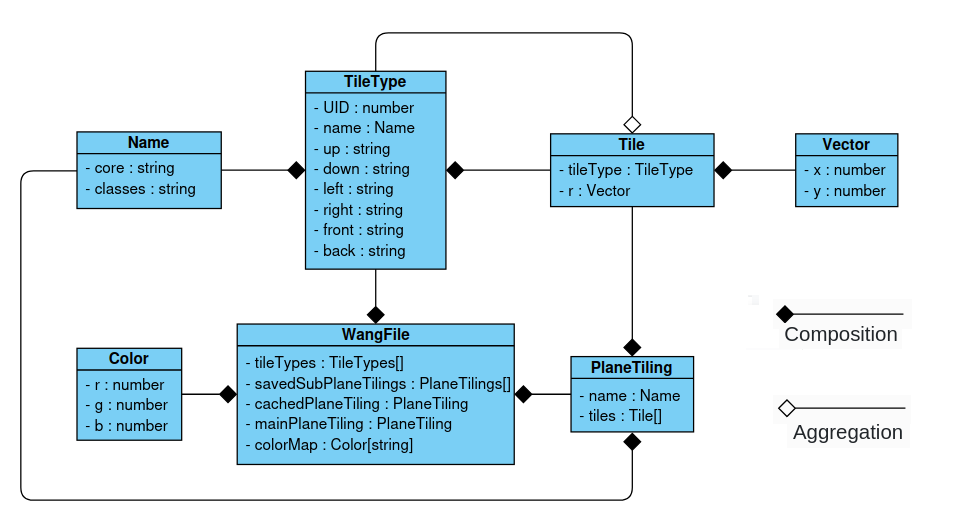
\includegraphics[width=6.4in]{figures/class-diagram.png}
	\caption{A UML class diagram describing the ontology underlying the system}
	\label{fig:1}
\end{figure}

A "tile type" refers to an entity that describes the adjacency rules which determine the legality of a tiling. A tile is a combination of a tile type with a position vector (a vector being a 2-tuple of real numbers). All tiles have positions which are aligned with the grid - each number in the 2-tuple is an integer.

A tiling is a collection of tiles in the x-y plane. The function mapping the tiles in a plane tiling to the set of tile types is surjective, but not necessarily injective. The function mapping the tiles in a tiling to the set of all possible positions is surjective, and not injective (since there are an infinite possible number of positions, and the number of tiles is finite).


Instead of using colors, the adjacency rules for tiles are enforced using strings. A significant advantage of using unicode strings instead of RGB 3-tuples is that a string is self-documenting. Another advantage is that strings are easy to tell apart from each other, unlike close shades of colors. Furthermore, the system is designed such that one can use it even if completely color-blind, albeit not as efficiently as if one can perceive colors perfectly.

A Wang file consists of a global set of tile types, a main tiling (on which most of the work is done), a cached tiling (used to implement resets while editing), a collection of sub tilings (which can be copied from and pasted into the main plane tiling) and a global color map that maps strings to colors. 

The entire state of the data is stored in the Wang file, and the Wang file can be exported and imported via JSON \cite{json} serialization. This process presents the following challenges:


\begin{itemize}
	\item JSON objects do not preserve references, so if multiple tiles have references to the same tile type object, deserialization creates two distinct but identical tile type objects. This is resolved using a readonly static UID associated with the tile type class, which is used to collapse references to identical tile types into a single object. 
	\item JSON objects carry only data and do not record non-static functions. This is resolved by replacing all non-static functions with static functions bound to the class, that takes an additional argument in place of "this" that the non-static function operates on.
	
\end{itemize}

\section*{Technology}

The software was designed to be a web-app, since this would allow it to be used by anyone with a browser. This also saves a lot of developer effort that would otherwise be spent in packaging the software for various operating systems and platforms.

\begin{figure}[h!tbp]
	\centering
	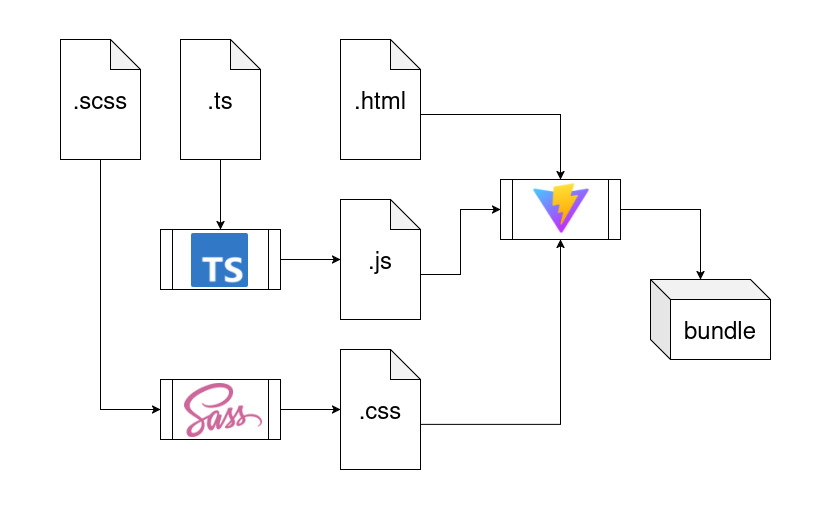
\includegraphics[width=6.4in]{figures/pipeline.png}
	\caption{The build pipeline, from the source files to the bundle}
	\label{fig:2}
\end{figure}

The following technology was used in the web-app:

\begin{itemize}
	\item HTML5 \cite{HTML5}, which is the industry standard for web development, used for the high-level structure of the web-app
	\item NPM \cite{npm} (Node package manager), used to install and maintain dependencies
	\item SASS \cite{sass} (Syntactically Awesome StyleSheets), which is a superset of CSS with additional syntactic sugar, used for styling the elements of the web-app
	\item TypeScript \cite{typescript}, which is a superset of JavaScript with a typing system, used for the describing the algorithms, data structures and UI interactions of the web-app
	\item three.js \cite{3js}, a package used to render objects in 3D using a WebGL context, without having to write any WebGL code directly
	\item Vite \cite{vite}, used to manage the compilation to CSS/JavaScript, minification \cite{minification}, tree-shaking \cite{tree} and bundling the web-app into a small, portable form
	\item Vitepress \cite{vitepress}, a static site generator \cite{ssg} used to generate the user manual from markdown \cite{markdown} source files
	\item GitHub actions, used as a CI/CD solution to build and publish the web-app incrementally
	\item GitHub pages, used to host the web-app online
\end{itemize}

In addition, the icons for the web-app were sourced from Google Material \cite{google-material} icons, downloaded as SVG images.


\section*{Algorithm}

\section*{Results}

A reference implementation for a two-state standalone clock is described below:

\begin{table}[h!tbp]
	\centering
	\caption{Adjacency rules for standalone-clock-0}
	{\footnotesize % reduce the font size for entire table
	\begin{tabular}{|l|r|}
	\hline
	  string & value \\
	\hline
	up & anything \\
	\hline
	down & anything \\
	\hline
	left & anything \\
	\hline
	right & anything \\
	\hline
	front & clock-1 \\
	\hline
	back & clock-0 \\
	\hline
	\end{tabular}
	}
	\end{table}

	\begin{table}[h!tbp]
		\centering
		\caption{Adjacency rules for standalone-clock-1}
		{\footnotesize % reduce the font size for entire table
		\begin{tabular}{|l|l|}
		\hline
		  string & value \\
		\hline
		up & anything \\
		\hline
		down & anything \\
		\hline
		left & anything \\
		\hline
		right & anything \\
		\hline
		front & clock-0 \\
		\hline
		back & clock-1 \\
		\hline
		\end{tabular}
		}
		\end{table}

The standalone clock consists of two states - clock-0 and clock-1. Each state only allows the other state to be placed next to it in the plane behind and in front of it along the z-axis. When moving along the z-axis, the tile at that location alternates between clock-0 and clock-1, which simulates a clock pulse.

\begin{figure}[h!tbp]
	\centering
	\begin{minipage}[b]{0.2\textwidth} 
		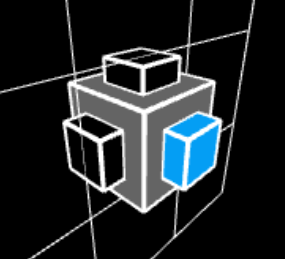
\includegraphics[width=\textwidth]{figures/0-clock.png}
				\subcaption*{standalone-clock-0} % Add subcaption text if desired, or use \subcaption* to suppress (a), (b), etc. labels
				\label{fig:2a}
	\end{minipage}
	~ %add desired spacing between images, e. g., ~, \quad, \qquad, \hfill etc.	
	\begin{minipage}[b]{0.2\textwidth} 
		
\includegraphics[width=\textwidth]{figures/1-clock.png}
				\subcaption*{standalone-clock-1} % Add subcaption text if desired, or use \subcaption* to suppress (a), (b), etc. labels
				\label{fig:2b}
	\end{minipage}
	\caption{standalone-clock: "clock-0" is mapped to grey and "clock-1" is mapped to cyan}
	\label{fig:2}
	\end{figure}


	Clocks that have different frequencies are implemented by adding more states - for instance, a clock that runs at half the base frequency has 4 states - clock-00, clock-01, clock-10 and clock-11. Other elements that don't have internal states that depend directly on time are given adjacency rules such that they propagate themselves.

	\begin{table}[h!tbp]
		\centering
		\caption{Adjacency rules for horizontal-wire-0}
		{\footnotesize % reduce the font size for entire table
		\begin{tabular}{|l|r|}
		\hline
		  string & value \\
		\hline
		up & anything \\
		\hline
		down & anything \\
		\hline
		left & 0 \\
		\hline
		right & 0 \\
		\hline
		front & wire \\
		\hline
		back & wire \\
		\hline
		\end{tabular}
		}
		\end{table}
	
		\begin{table}[h!tbp]
			\centering
			\caption{Adjacency rules for horizontal-wire-1}
			{\footnotesize % reduce the font size for entire table
			\begin{tabular}{|l|l|}
			\hline
			  string & value \\
			\hline
			up & anything \\
			\hline
			down & anything \\
			\hline
			left & anything \\
			\hline
			right & anything \\
			\hline
			front & wire \\
			\hline
			back & wire \\
			\hline
			\end{tabular}
			}
			\end{table}

For all such elements, rotations and reflections require different tile types, though the relationships between the adjacency rules of rotated and reflected tile types enables the web app to generate them automatically, without requiring the user to manually enter all the rules.

\begin{figure}[h!tbp]
	\centering
	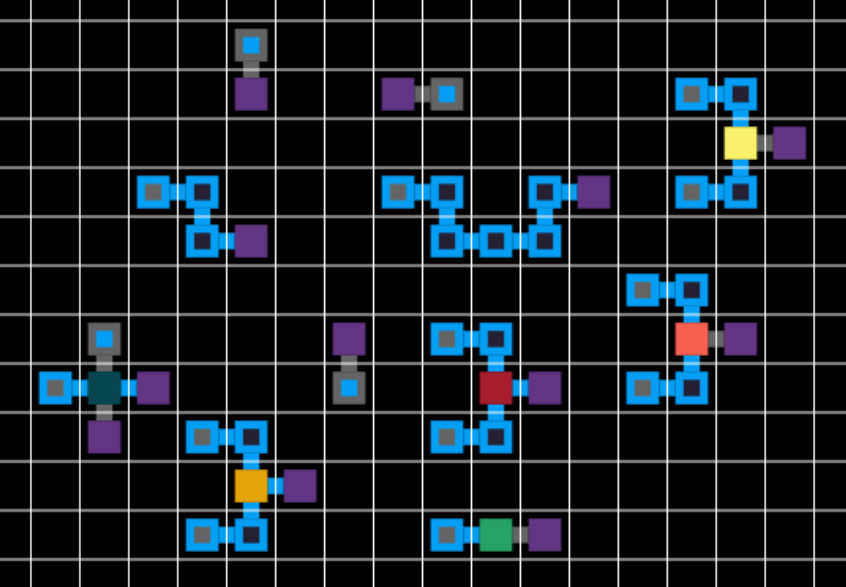
\includegraphics[width=6.4in]{figures/gates-wires-clocks.png}
	\caption{Logic gates: AND (red), OR (deep-yellow) NOT (green), NAND (orange), NOR (light-yellow), wires (grey/cyan), junctions (deep cyan), clocks,  and sinks (purple)}
	\label{fig:2}
\end{figure}


\section*{Future work}

The following circuits can be added to the project:

\begin{itemize}
	\item D-flip-flops, constructed either as a standalone tile or from two D-latches. This requires a consistent translation of the notion of rising and falling edges to a system with discrete time, which requires research into variants of flip-flops
	\item shift-registers, built from T-flip-flops. This allows one to build clocks of arbitrary frequencies without creating a large number of clock tiles to represent each state
	\item Single-tile wires with more than two states, which can be used to transmit signals effectively, when coupled with multiplexers and demultiplexers
	\item A 7-segment display, using a $3 x 5$ grid of screen tiles, with each tile having 10 states, though making 150 manually using the current UI is tedious
\end{itemize}

The following UI improvements can be made to the project:

\begin{itemize}
	\item An implementation of the pause/play functionality, which is currently left unimplemented due to difficulties involved with managing the animation framerate with the system clock (for security reasons, most browsers do not allow scripts to access the exact time on the system clock)
	\item A custom console, to display errors and warnings at different levels of verbosity (at present, all such messages show up in the console provided with the developer tools of the browser)
	\item An input console to allow the programmatic manipulation of the Wang file, to automate tedious tasks
	\item Collapsible classes in the search results, making a tree-like structure that's easier to navigate than scrolling over all the results
	\item A graphical representation of the illegality of the tiling (for instance, using red circles to point out areas where the adjacency rules are violated)
	\item Integrating the main editor with three.js, allowing the user to manipulate the main tiling using orbit controls (currently unimplemented due to problems with mixing dynamic resizing with the WebGL API of three.js)
\end{itemize}

% %%%%%%%%%%%%%%%%%%%%%%%%%%%%%%%%%%%%%%%%%%%
% \section*{Some Guide on Content}

% % And don't try to mix and match numbered and unnumbered sections; it's one or the other.

% Let's start with some advice on the subject matter and content of a
% Bridges paper, since this should be an author's first concern. The
% Bridges Proceedings are considered a refereed journal, and as such we
% are trying to maintain quality standards that will make its papers count
% in academic personnel reviews and promotion cases. Thus, most
% importantly, every paper should present some novel achievements,
% experiments, artwork, and/or insights by the authors. General reviews or
% tutorials, cobbled together from various blogs or Wikipedia pages are
% not appropriate. Also, keep in mind that the number of pages in the
% Proceedings as well as your presentation time at the conference are
% limited; so choose a scope for your presentation that fits into these
% constraints.

% \textbf{Regular papers} should be either 8 or 6 pages, including references. Every paper should nicely
% fill an even number of pages without a lot of wasted white space, so
% that we can make optimal use of the Proceedings pages and start every
% paper on a right-hand page.

% \textbf{Short papers}, which have a later submission deadline, should be
% 4 or 2 pages long, including references. Here it is particularly important to focus 
% on just one or two novel ideas and results. Short papers are not a good medium
% to give tutorial introductions or cursory reviews over a domain that could be the 
% subject of one or more books. Also, this is not the place to give preliminary ideas 
% on new teaching experiments, or to present intuitive hunches how some classical 
% artwork might be analyzed in a novel way. A Bridges paper should only be submitted 
% after the experiments or novel analysis have been performed and when concrete results are available.

% The program committee has found that certain types of papers almost always 
% need to be rejected: papers on numerology or work that extracts numbers or 
% ratios from artwork or architecture. A somewhat ``fuzzy'' search for the Golden 
% Ratio (or any other ratio) will almost always produce some hits (a simple matter of 
% statistics). However, such coincidences do not tell us anything about the method 
% or intent of the creator of those artifacts, unless there is some other
% compelling evidence, such as auxiliary lines or notes that explicitly
% state what the artist or architect was doing.

% Please write your paper in such a way that attendees with a general
% education can follow your discourse without the need to look up several
% references to find out what the main gist is of your paper. Skip lengthy
% sections on \emph{background} and \emph{previous work} and instead give
% clear and detailed explanations on your novel contributions, ideally
% well-supported with diagrams and/or images.


% %%%%%%%%%%%%%%%%%%%%%%%%%%%%%%%%%%%%%%%%%%%
% \section*{Use of this Template}

% \noindent If you are writing your paper using \LaTeX, please use a
% copy of the source \texttt{.tex} file for this document as your starting point. Some 
% useful \LaTeX\ resources are \cite{Chang, Gratzer}. This template (with its accompanying 
% style file) has been set with the proper paper size and all the necessary \emph{styles} for
% proper formatting. Just replace the text in this file with your own text. Also substitute 
% your own images for the figures in this template, either as an individual figure like 
% Figure \ref{fig:1}, or, alternatively, as in the composite Figure \ref{fig:2}. Each figure is then 
% followed by a \verb|\caption|.

% \begin{figure}[h!tbp]
% 	\centering
% 	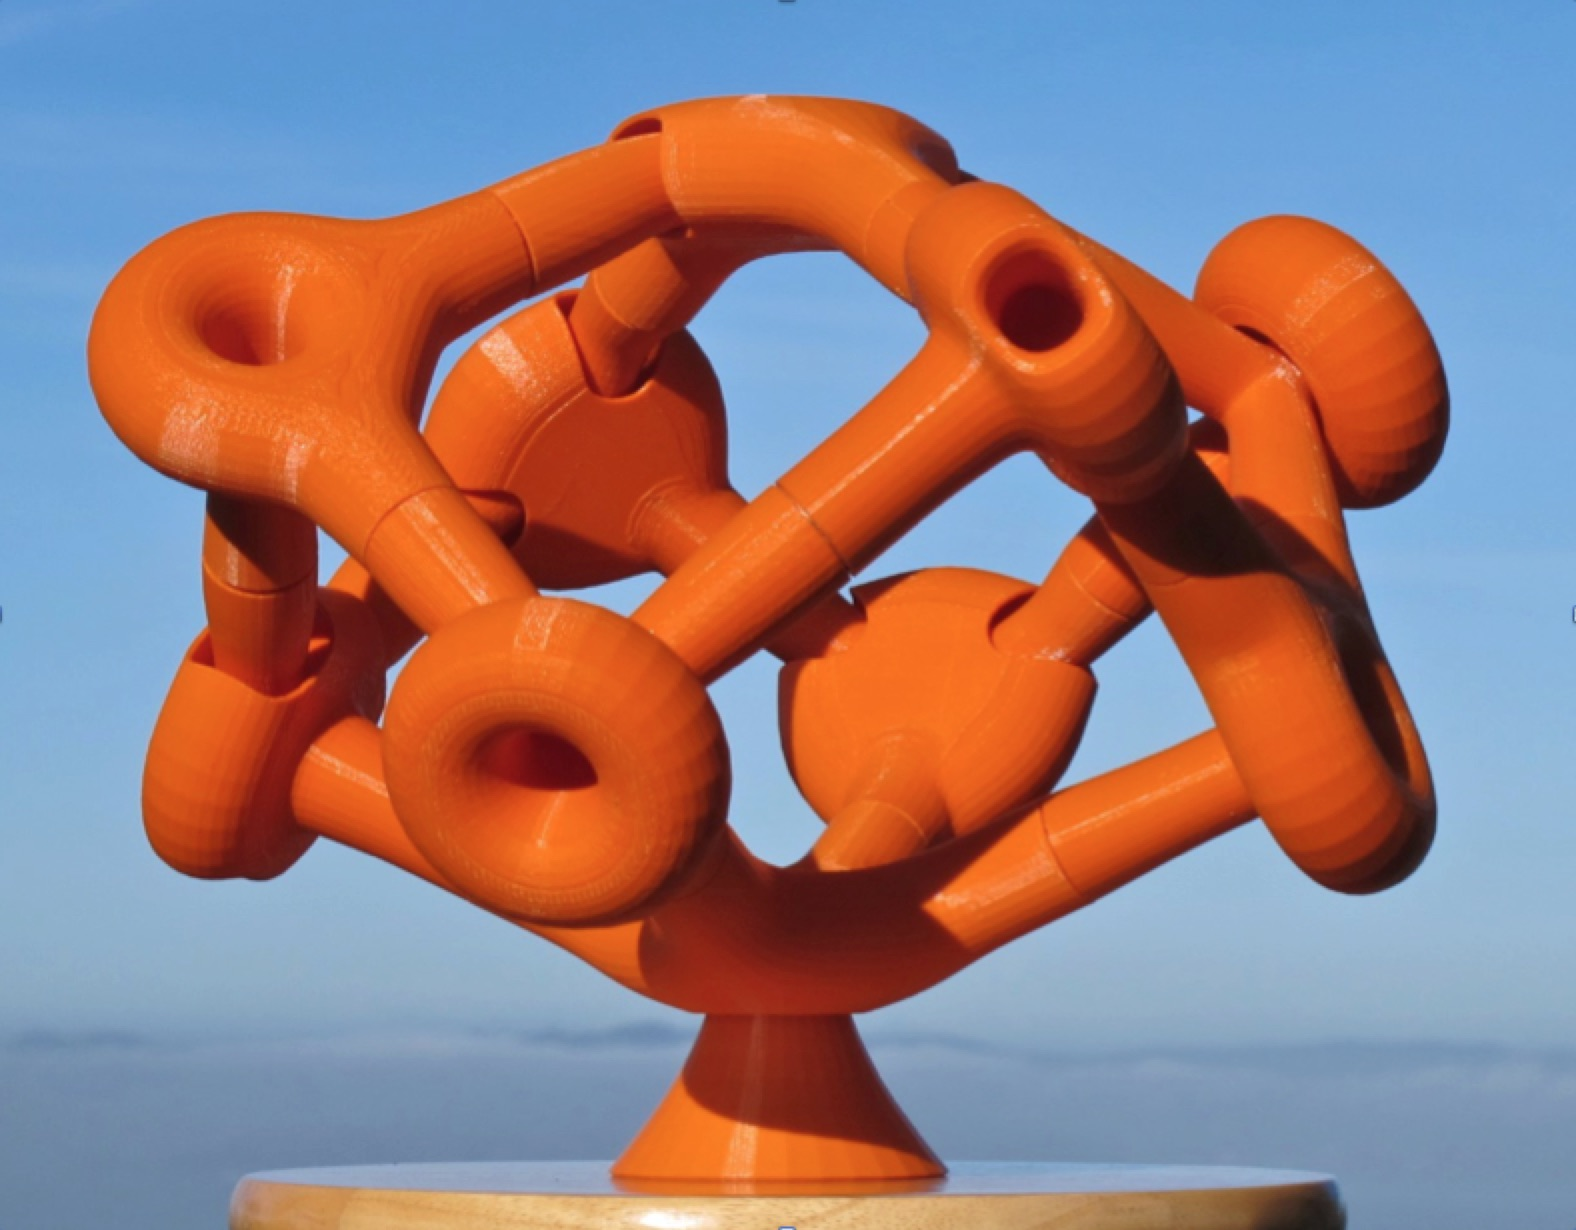
\includegraphics[width=2.4in]{figures/figure1.jpg}
% 	\caption{An individual figure \cite{Sequin2016}. Make it large enough so that necessary 
% 	details can be seen.\\ Fine-tune its size, so that you obtain convenient page breaks.}
% 	\label{fig:1}
% \end{figure}



% %%%%%%%%%%%%%%%%%%%%%%%%%%%%%%%%%%%%%%%%%%%
% \section*{Paper Size, Margins, and Styles}

% The Proceedings will be printed using US Letter size paper (8.5 by 11
% inches) as in this document. If you are working outside the USA, please
% check that you have not used A4 paper, which may be the default in your
% country. Do not insert page numbers, headers or footers; these will be
% inserted later at the publishing stage.

% This template has the proper styles set in the \texttt{bridges.sty} file. 
% The result should conform to the following specifications: On the first page, 
% the distance from the top edge of the paper to the first line of the title should 
% be 3~cm ($1+3/16$ inches). On the second and subsequent pages, the distance 
% from the top edge of the paper to the top of the first line of type should be
% 2.5~cm (1~inch). The widths of the margins on left and right edges and
% at the bottom of the page should all be 2.5~cm (1~inch) as well.

% The font is \emph{Times New Roman}. The text of the main body,
% as well as the figure captions use size 11~pt. Section headings,
% authors, and affiliations are size 12~pt. Paper title is 16~pt. Abstract
% is 9~pt. Use this template to see what items are printed in \textbf{bold
% face} or in \emph{italics}. Use italics for emphasis, rather than blood face (which reads like yelling.)
% Mathematical expressions are typeset 
% in the same font as the body text, as in $\sqrt{b^2-4ac}$. 

% There should be no indentation for the first paragraph after a section heading. Subsequent paragraphs in that section will be indented. The style file will attend to this behavior, and will also justify text to both the left and right margins. 

%%%%%%%%%%%%%%%%%%%%%%%%%%%%%%%%%%%%%%%%%%%
% \section*{Figures and Tables}

% You must obtain permission and provide attribution to use any copyrighted material. 
% Images should be high quality. The proceedings will be produced in full color both online and in print.
% But be careful that your images do not make your final PDF larger than 10~Mb;
% in that case you may need to downsample your image files to reduce their size.

% To insert a figure, use the \emph{figure} environment. For this template, all
% image files are placed in the \texttt{images} folder, located in the directory containing the source 
% \texttt{.tex} file. Figure captions will be numbered and labeled automatically. Hence the boldface text 
% ``\textbf{Figure 1:}'' does not need to be typed as part of the figure caption, nor does the 
% italic font style need to be specified; these are handled automatically by the Bridges style file.

% Figure \ref{fig:2} shows how to format and caption a figure with multiple panels. 
% Here we use the \emph{subcaption} package, which enables the \verb|\subcaption| 
% command. Leave the subfigure captions blank to automatically label the panels 
% (a), (b), etc. We ensure that the full figure does not exceed the width of a full line 
% of text by setting the width of each individual panel to be an appropriate proportion of the 
% \verb|\textwidth|.

% \begin{figure}[h!tbp]
% \centering
% \begin{minipage}[b]{0.2\textwidth} 
% 	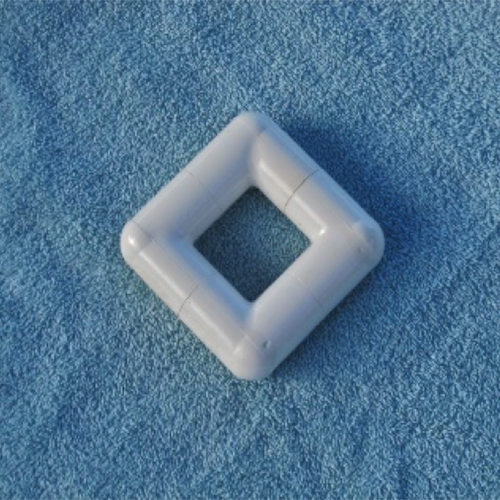
\includegraphics[width=\textwidth]{figures/figure2a.png}
%         	\subcaption{} % Add subcaption text if desired, or use \subcaption* to suppress (a), (b), etc. labels
%         	\label{fig:2a}
% \end{minipage}
% ~ %add desired spacing between images, e. g., ~, \quad, \qquad, \hfill etc.	
% \begin{minipage}[b]{0.2\textwidth} 
% 	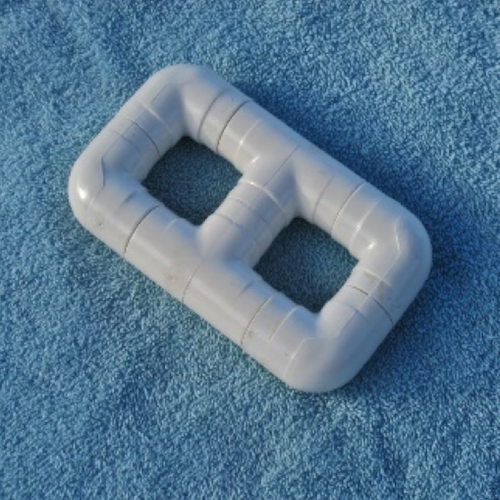
\includegraphics[width=\textwidth]{figures/figure2b.png}
%         	\subcaption{} % Add subcaption text if desired, or use \subcaption* to suppress (a), (b), etc. labels
%         	\label{fig:2b}
% \end{minipage}
% ~ %add desired spacing between images, e. g., ~, \quad, \qquad, \hfill etc.	
% \begin{minipage}[b]{0.2\textwidth} 
% 	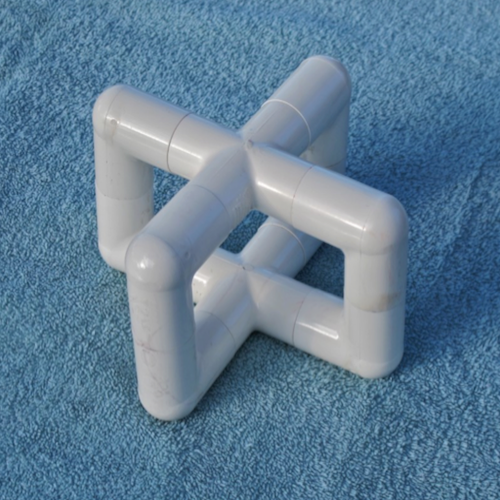
\includegraphics[width=\textwidth]{figures/figure2c.png}
%         	\subcaption{} % Add subcaption text if desired, or use \subcaption* to suppress (a), (b), etc. labels
%         	\label{fig:2c}
% \end{minipage}
% ~ %add desired spacing between images, e. g., ~, \quad, \qquad, \hfill etc.	
% \begin{minipage}[b]{0.2\textwidth} 
% 	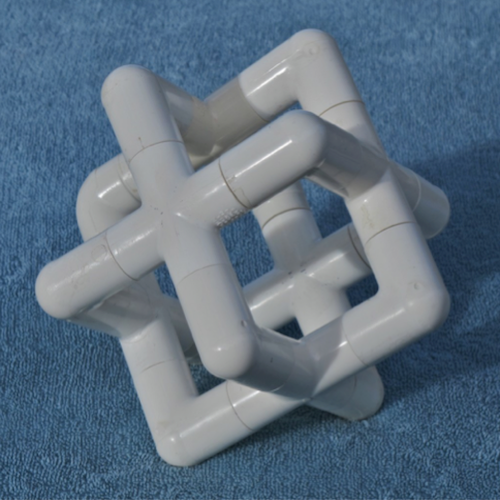
\includegraphics[width=\textwidth]{figures/figure2d.png}
%         	\subcaption{} % Add subcaption text if desired, or use \subcaption* to suppress (a), (b), etc. labels
%         	\label{fig:2d}
% \end{minipage}
% \caption{Orientable handle-bodies made from PVC pipe components:  (a) simple torus of genus 1, \\
% (b) 2-hole torus of genus 2,  (c) handle-body of genus 3,  (d) handle-body of genus 7.}
% \label{fig:2}
% \end{figure}
% % NOTE: As an alternative, you could use \caption instead of \subcaption for the individual panels, 
% % and remove the composite \caption at the bottom. This will produce separate side-by-side figures,
% % each with its own Figure number.


% Tables are mostly treated just like figures, except that the caption is 
% is placed \emph{above} the table body. This is accomplished by placing the 
% \verb|\caption| before the table data. In this example we reduce the font size 
% in the \emph{tabular} environment so the table fits within the margins. 
% All figures and tables must be referenced and explained in the main text, and they must
% not bleed into the margins.

% \begin{table}[h!tbp]
% \centering
% \caption{Number of Topologically Different Linkings of Two Cube-Frames.}
% {\footnotesize % reduce the font size for entire table
% \begin{tabular}{|l|l|l|l|l|l|r|}
% \hline
%   & 2 edge-loops & 3 edge-loops & 4 edge-loops & 5 edge-loops & 6 edge-loops & total \\
% \hline
% 2 edge-loops & 2sm, 1dm & & & & & 3  \\
% \hline
% 3 edge-loops & 0 & 1sm, 1sp, 2sc, 2dm & & & & 6 \\
% \hline
% 4 edge-loops & 0 & 2dc & 1sm, 10 sc, 2dm, 10dc & & & 25\\  
% \hline
% 5 edge-loops & 0 & 0 & 1dm, 20dc & 16sc, 3dm, 1dp, 24dc & & 65  \\  
% \hline
% 6 edge-loops & 0 & 0 &  3dm, 2dc & 26dc & 14sc & 45\\  
% \hline
%  & & & & & \multicolumn{1}{r|}{total:} & 144\\
%  \hline
%  & \multicolumn{2}{c|}{s: swap symmetry} & \multicolumn{2}{c|}{m: mirror symmetry} & & \\
%  \hline
%  & \multicolumn{2}{c|}{d: different roles for} & \multicolumn{2}{c|}{c: chiral configuration} & \multicolumn{2}{r|}{date: 1/20/2016}   \\
%  \hline
%  & \multicolumn{2}{c|}{the two frames} & \multicolumn{2}{c|}{p: pseudo chirality} & & \\
%  \hline
% \end{tabular}
% }
% \end{table}


%%%%%%%%%%%%%%%%%%%%%%%%%%%%%%%%%%%%%%%%%%%
% \section*{Sections and Subsections}

% Important words should be capitalized in your paper's title and section
% headings, while conjunctions (e.g., ``and'' / ``or'') and prepositions
% (e.g., ``of'' / ``with'') begin with a lower case letter. Avoid most punctuation 
% (one colon or comma is acceptable). Do not end a lone title or section heading with a period. 
% For section headings use \verb|\section*|. Do not use numbered sections
% unless you refer to a section by number rather than title in the text. 
% If you must have your sections numbered use the \verb|\section| 
% command. For any Bridges paper, it would probably be excessive to use 
% more than two levels of hierarchy in your document. In all papers the \textbf{Abstract}, 
% \textbf{Acknowledgments}, and \textbf{References} headings are unnumbered 
% sections.

% %%%%%%%%%%%%%
% \subsection*{Subsections}

% If needed, you may introduce subsections using the command
% \verb|\subsection*|. Subsections are never numbered. Subsection titles 
% are 11~pt, left justified, bold, and italicized.

% %%%%%%%%%%%%%
% \subsection*{Vertical Spacing and Page Breaks}

% The various styles for headings and paragraphs come with their own
% built-in vertical spacing. By default they should result in a good-looking layout. 
% But occasionally it is necessary to change vertical spacing a little in order to 
% avoid inconvenient page breaks. Try to avoid the last line of a paragraph appearing 
% at the beginning of the next page and don't leave a section title on a separate page 
% from what follows. Feel free to introduce \verb|\vspace*|
% or \verb|\pagebreak| to improve layout.

% %%%%%%%%%%%%%
% \subsection*{Wrap-up}

% % Define BibTeX command for typesetting its logo as it appears the following paragraph -- Feel free 
% % to comment this out or delete entirely in your paper.
% \def\BibTeX{{\rm B\kern-.05em{\sc i\kern-.025em b}\kern-.08em
%     T\kern-.1667em\lower.7ex\hbox{E}\kern-.125emX}}

% The paper should end with a brief section that provides some \textbf{Summary and Conclusions}. 
% This may be followed by \textbf{Acknowledgments} (optional) and \textbf{References}. Only list 
% references that you cite in your paper. List all references alphabetically by last name of first 
% author and number them sequentially. When citing references in the text, use \verb|\cite|, as in: 
% ``see Coxeter \cite{Coxeter}'' or just insert ``\cite{Coxeter}'' after the corresponding quote. 
% See the references for correct article \cite{EJCx,Coxeter}, book \cite{Gratzer}, and Bridges 
% Conference Proceedings \cite{Sequin2016} citations. Since Bridges papers typically have only 
% a few references, we do not require or even recommend that you use \BibTeX, but of course 
% you are free to do so. Examples and templates for other types of references can be found in the Guidelines for References section of the Paper Formatting webpage. Don't insert links to references in the body of the paper. 


% %%%%%%%%%%%%%%%%%%%%%%%%%%%%%%%%%%%%%%%
% \section*{Writing Style and Final Format}

% There is no need to use only the passive voice, often encountered in
% some formal academic journals. It is perfectly acceptable to use the
% first person ``I'' when talking about your own artistic endeavors, and
% the inclusive, academic ``we'' works well for more formal statements.

% To submit your paper via EasyChair \cite{easychair}, 
% you will have to convert it into a PDF (Portable Document Format) file and that file must not exceed 10 MB.
% Papers will appear in the online Bridges Archives and in print in full color.



%%%%%%%%%%%%%
% \section*{Summary and Conclusions}

% Please adhere to the style incorporated in this template, \emph{except} your paper
% must end after 2, 4, 6, or 8 pages, \emph{including} references. Substantive
% deviations from this style are grounds for rejecting your paper without
% any detailed review.

\section*{LLM disclosure}

No LLMs were used in the generation of this report or the user manual for the web-app. However, when writing the code for the web-app, the involvement of LLMs is difficult to quantify and disentangle from the code written by a human, for the following reasons:

\begin{itemize}
	\item Development often involves copying and pasting code from online forums such as StackOverflow. The source of the content on such forums cannot be guaranteed to be written by a human, unless accompanied with a timestamp preceding the release of popular LLMs like ChatGPT.
	\item Since search engines integrate AI assistance with their service, searching for a topic results in the user being exposed to an AI-generated answer that appears before every search result. This could subtly influence the thought-process of the user, guiding them toward certain implementations and solutions.
	\item Popular code-editors like Copilot now integrate agentic coding assistants powered by LLMs, which autocomplete code snippets and generate functions from comments. Though no such editor has been used in the development of this web-app, it is often the case that the coder does not have direct control over what editor they are allowed to use.
\end{itemize}


%%%%%%%%%%%%%%%%%%%%%%%%%%%%%%%%%%%%%%%
% \section*{Acknowledgements}

% Suggestions on how the clarity and usefulness of this guide could be
% enhanced would be gladly accepted.

%%%%%%%%%%%%%%%%%%%%%%%%%%%%%%%%%%%%%%%
% References %
    
{\setlength{\baselineskip}{13pt} % tighten line spacing for bibliography
\raggedright				% no right justification for References
\begin{thebibliography}{99}

% \bibitem{Chang}
% W. Chang. \LaTeX\ \textit{Cheat Sheet}. 2014. \url{http://wch.github.io/latexsheet/}.

% \bibitem{EJCx}
% M.\ Chladn\'y and M.\ \v Skoviera. ``Factorisation of Snarks.'' \textit{Electronic Journal
% of Combinatorics}, vol.~17, no.~1, R32, 2010.
% \url{http://www.combinatorics.org/Volume_17/PDF/v17i1r32.pdf}.

% \bibitem{Coxeter} H.\ S.\ M.\ Coxeter. ``The Non-Euclidean Symmetry of Escher's Picture
% Circle Limit III.'' \textit{Leonardo}, vol.~12, no.~1, 1979, pp.~19--25.

% \bibitem{easychair} EasyChair. Log in page. \url{https://easychair.org/account/signin.cgi}.

% \bibitem{Gratzer} G.\ Gr\"atzer. \textit{More Math Into} \LaTeX, 4th ed. Springer, 2007.

% \bibitem{Sequin2016} C.\ H.\ S\'equin. ``From Klein Bottles to Modular Super-Bottles.'' 
% \textit{Bridges Conference Proceedings}, Jyv\"askyl\"a, Finland, Aug. 9--13,
% 2016, pp.~41--48. \url{http://archive.bridgesmathart.org/2016/bridges2016-41.html}.


\bibitem{manual} User manual, GitHub pages. \url{https://mathewkj2048.github.io/Wang-cube-circuit-simulator-user-manual}

\bibitem{web-app} Web app, GitHub pages. \url{https://mathewkj2048.github.io/Wang-cube-circuit-simulator/}

\bibitem{web-app-source} Web app source code, GitHub \url{https://github.com/MathewKJ2048/Wang-cube-circuit-simulator}

\bibitem{wang-file} Clocks, wires and logic gates, GitHub \url{https://github.com/MathewKJ2048/Wang-cube-circuit-simulator/tree/main/Wang-files}

\bibitem{Merrel} Merrel, Paul. ``Example-based model synthesis'' \textit{Proceedings of the 2007 Symposium on Interactive 3D Graphics and Games}, 2007, pp.105--112 \url{https://doi.org/10.1145/1230100.1230119}

\bibitem{tree} Tree-shaking, MDN web docs. \url{https://developer.mozilla.org/en-US/docs/Glossary/Tree_shaking}

\bibitem{minification} Minification, MDN web docs. \url{https://developer.mozilla.org/en-US/docs/Glossary/Minification}

\bibitem{HTML5} HTML5,  MDN web docs. \url{https://developer.mozilla.org/en-US/docs/Glossary/HTML5}

\bibitem{sass} Documentation, sass-lang. \url{https://sass-lang.com/documentation/}

\bibitem{typescript} TypeScript,  MDN web docs. \url{https://developer.mozilla.org/en-US/docs/Glossary/TypeScript}

\bibitem{vite} Vite. \url{https://vite.dev/}

\bibitem{ssg} Static Site Generator, MDN web docs. \url{https://developer.mozilla.org/en-US/docs/Glossary/SSG}

\bibitem{npm} Node Package Manager. \url{https://docs.npmjs.com/about-npm}

\bibitem{markdown} How to write in Markdown, MDN web docs. \url{https://developer.mozilla.org/en-US/docs/MDN/Writing_guidelines/Howto/Markdown_in_MDN}

\bibitem{json} JavaScript Object Notation. \url{https://www.json.org/json-en.html}

\bibitem{vitepress} Vitepress \url{https://vitepress.dev/}

\bibitem{3js} three.js \url{https://threejs.org/}

\bibitem{google-material} Google Material icons. \url{https://fonts.google.com/icons}



\end{thebibliography}
} % end setlength, raggedright
   
\end{document}